\documentclass[english,11pt,usenames,dvipsnames]{beamer}

\DeclareMathOperator{\Cov}{Cov}
\DeclareMathOperator{\Var}{Var}
\DeclareMathOperator{\E}{\mathbb{E}}
\DeclareMathOperator{\Proba}{\mathbb{P}}

\newcommand{\Covb}[2]{\ensuremath{\Cov\!\left[#1,#2\right]}}
\newcommand{\Eb}[1]{\ensuremath{\E\!\left[#1\right]}}
\newcommand{\Pb}[1]{\ensuremath{\Proba\!\left[#1\right]}}
\newcommand{\Varb}[1]{\ensuremath{\Var\!\left[#1\right]}}

% norm
\newcommand{\norm}[1]{\| #1 \|}

\newcommand{\indep}{\rotatebox[origin=c]{90}{$\models$}}





\usepackage{mathptmx,amsmath,amssymb,graphicx,bibentry,bbm,babel,ragged2e}

\makeatletter

\newcommand{\noun}[1]{\textsc{#1}}
\newcommand{\jitem}[1]{\item \begin{justify} #1 \end{justify} \vfill{}}
\newcommand{\sframe}[2]{\frame{\frametitle{#1} #2}}

\newenvironment{centercolumns}{\begin{columns}[c]}{\end{columns}}
%\newenvironment{jitem}{\begin{justify}\begin{itemize}}{\end{itemize}\end{justify}}

\usetheme{Warsaw}
\setbeamertemplate{footline}[text line]{}
\setbeamercolor{structure}{fg=purple!50!blue, bg=purple!50!blue}

\setbeamersize{text margin left=15pt,text margin right=15pt}

\setbeamercovered{transparent}

\setbeamertemplate{headline}{}
\setbeamertemplate{footline}[frame number]
\setbeamertemplate{navigation symbols}{}

\@ifundefined{showcaptionsetup}{}{%
 \PassOptionsToPackage{caption=false}{subfig}}
\usepackage{subfig}

\usepackage[utf8]{inputenc}
\usepackage[T1]{fontenc}


\usepackage{tikz}

\usepackage{multirow}

\usepackage{mdframed}

%\usepackage[usenames,dvipsnames]{pstricks}
%\usepackage{auto-pst-pdf}


%\usepackage[dvipsnames]{xcolor}

\usepackage{threeparttable}


\makeatother

\begin{document}


\title{Linking Microsimulation and LUTI models}

%\author{J.~Raimbault$^{1,2,3}$\\
%\texttt{juste.raimbault@iscpif.fr}
%}


%\institute{$^{1}$UPS CNRS 3611 ISC-PIF\\
%$^{2}$CASA, UCL\\
%$^{3}$UMR CNRS 8504 G{\'e}ographie-cit{\'e}s
%}

\date{11/06/2019}

\frame{\maketitle}



%\section{Introduction}


\sframe{Context}{

\textit{We try to couple these models because we were asked to, but is it relevant and will it be used ?}

\bigskip

$\rightarrow$ how is the approach relevant ?

\medskip

$\rightarrow$ what are we dealing with exactly ?

\medskip

$\rightarrow$ theoretical and technical prospects, feasibility

}

\sframe{Outline}{
\tableofcontents
}

\section{Literature mapping}
% global overview with citation maps 
% (different use of microsim)


\sframe{Citation network analysis}{

\justify

 % - very different approaches with same name ?
 % - potential/relevance to couple approaches ?

 \begin{itemize}
 	\item Urban modeling in general very broad on models used and how to name/describe them
 	\item What are existing existing/potential connections between approaches?
 \end{itemize}
 
 \bigskip

 $\rightarrow$ \textit{a systematic review and citation network exploration around our main entries (microsimulation and luti)}

 \medskip
 
 Currently :
 
 \begin{itemize}
 \item Extended/rewrote a bibliographic data collection and management library (java) to get citation data from google scholar (parallel collection, mongodb storage) \cite{raimbault2019exploration}
 \item Citation network analysis (4.67e5 papers, 8.34e5 citation links): endogenous disciplines and their positioning, evolution of communities in time
 \end{itemize}
 
 

}

\sframe{Coverage of the citation network}{
  
  \textit{Robustness of the corpus to the construction method (keyword request): majority coverage for each request}
  
  \medskip
  
  \centering
  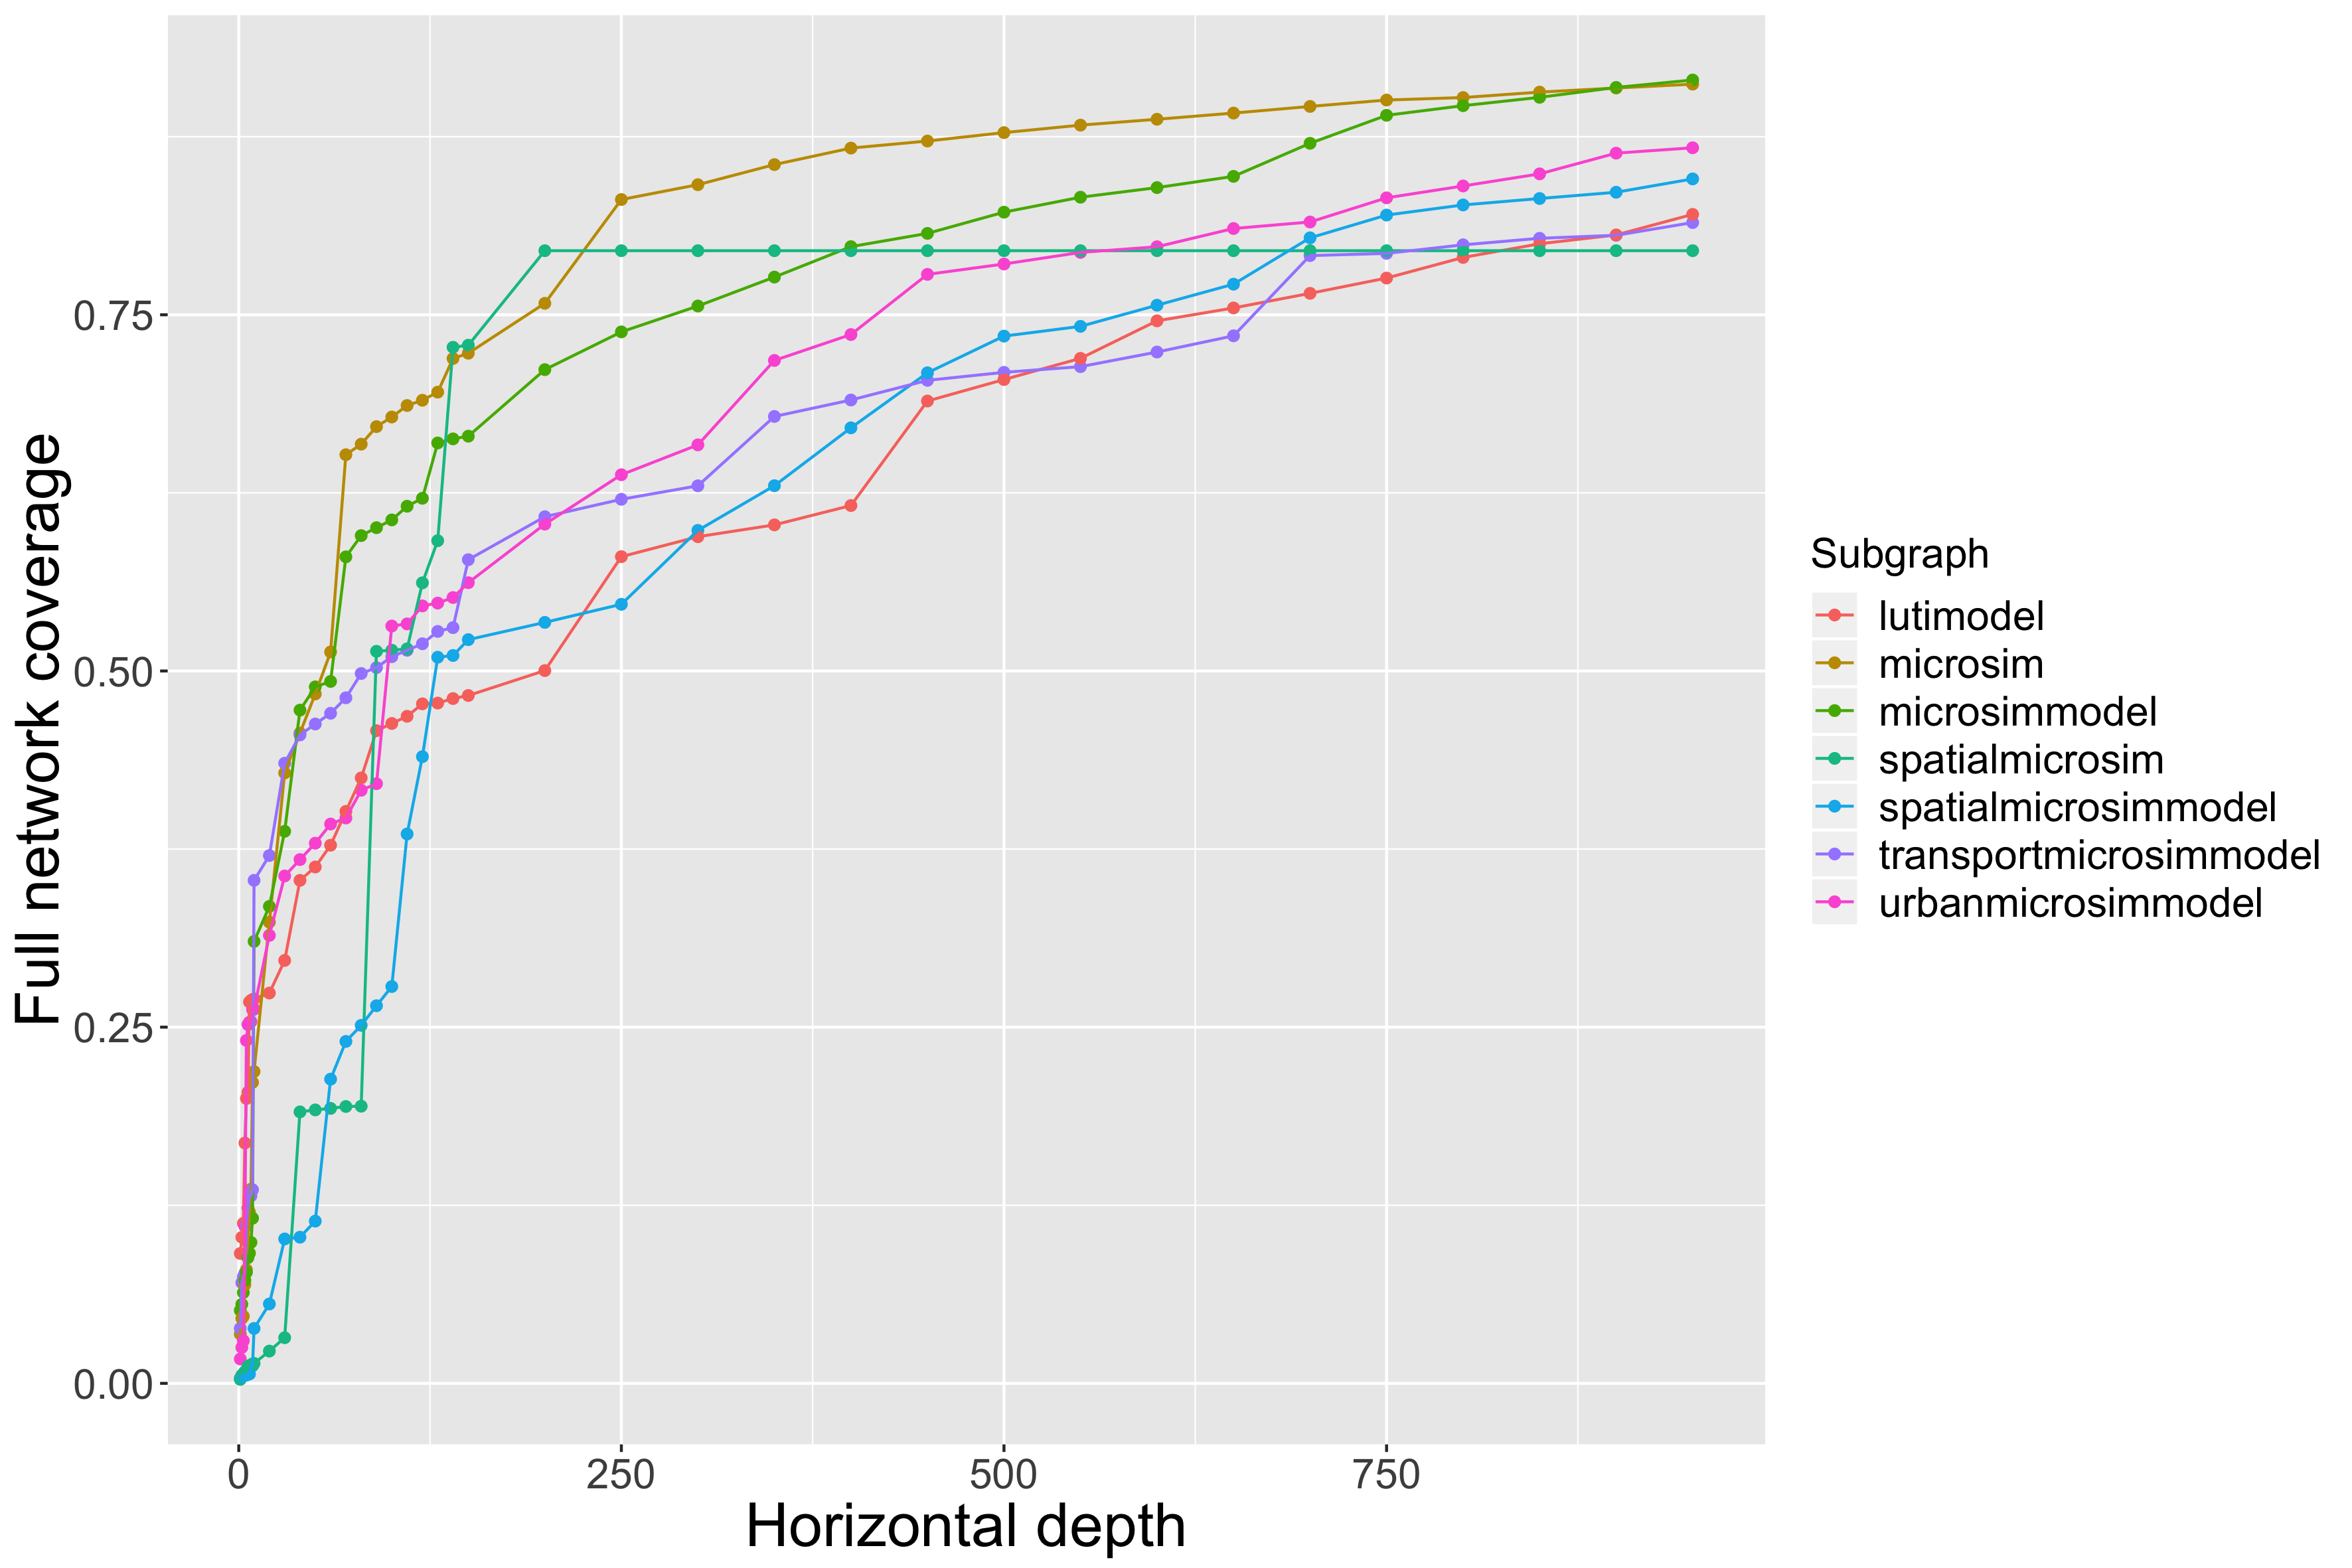
\includegraphics[height=0.8\textheight]{figures/coverage_subnws}
  
}

\sframe{Sensitivity analysis}{

\textit{Multiobjective optimization of network structure on the parameter for query answer kept}

\medskip

\centering
 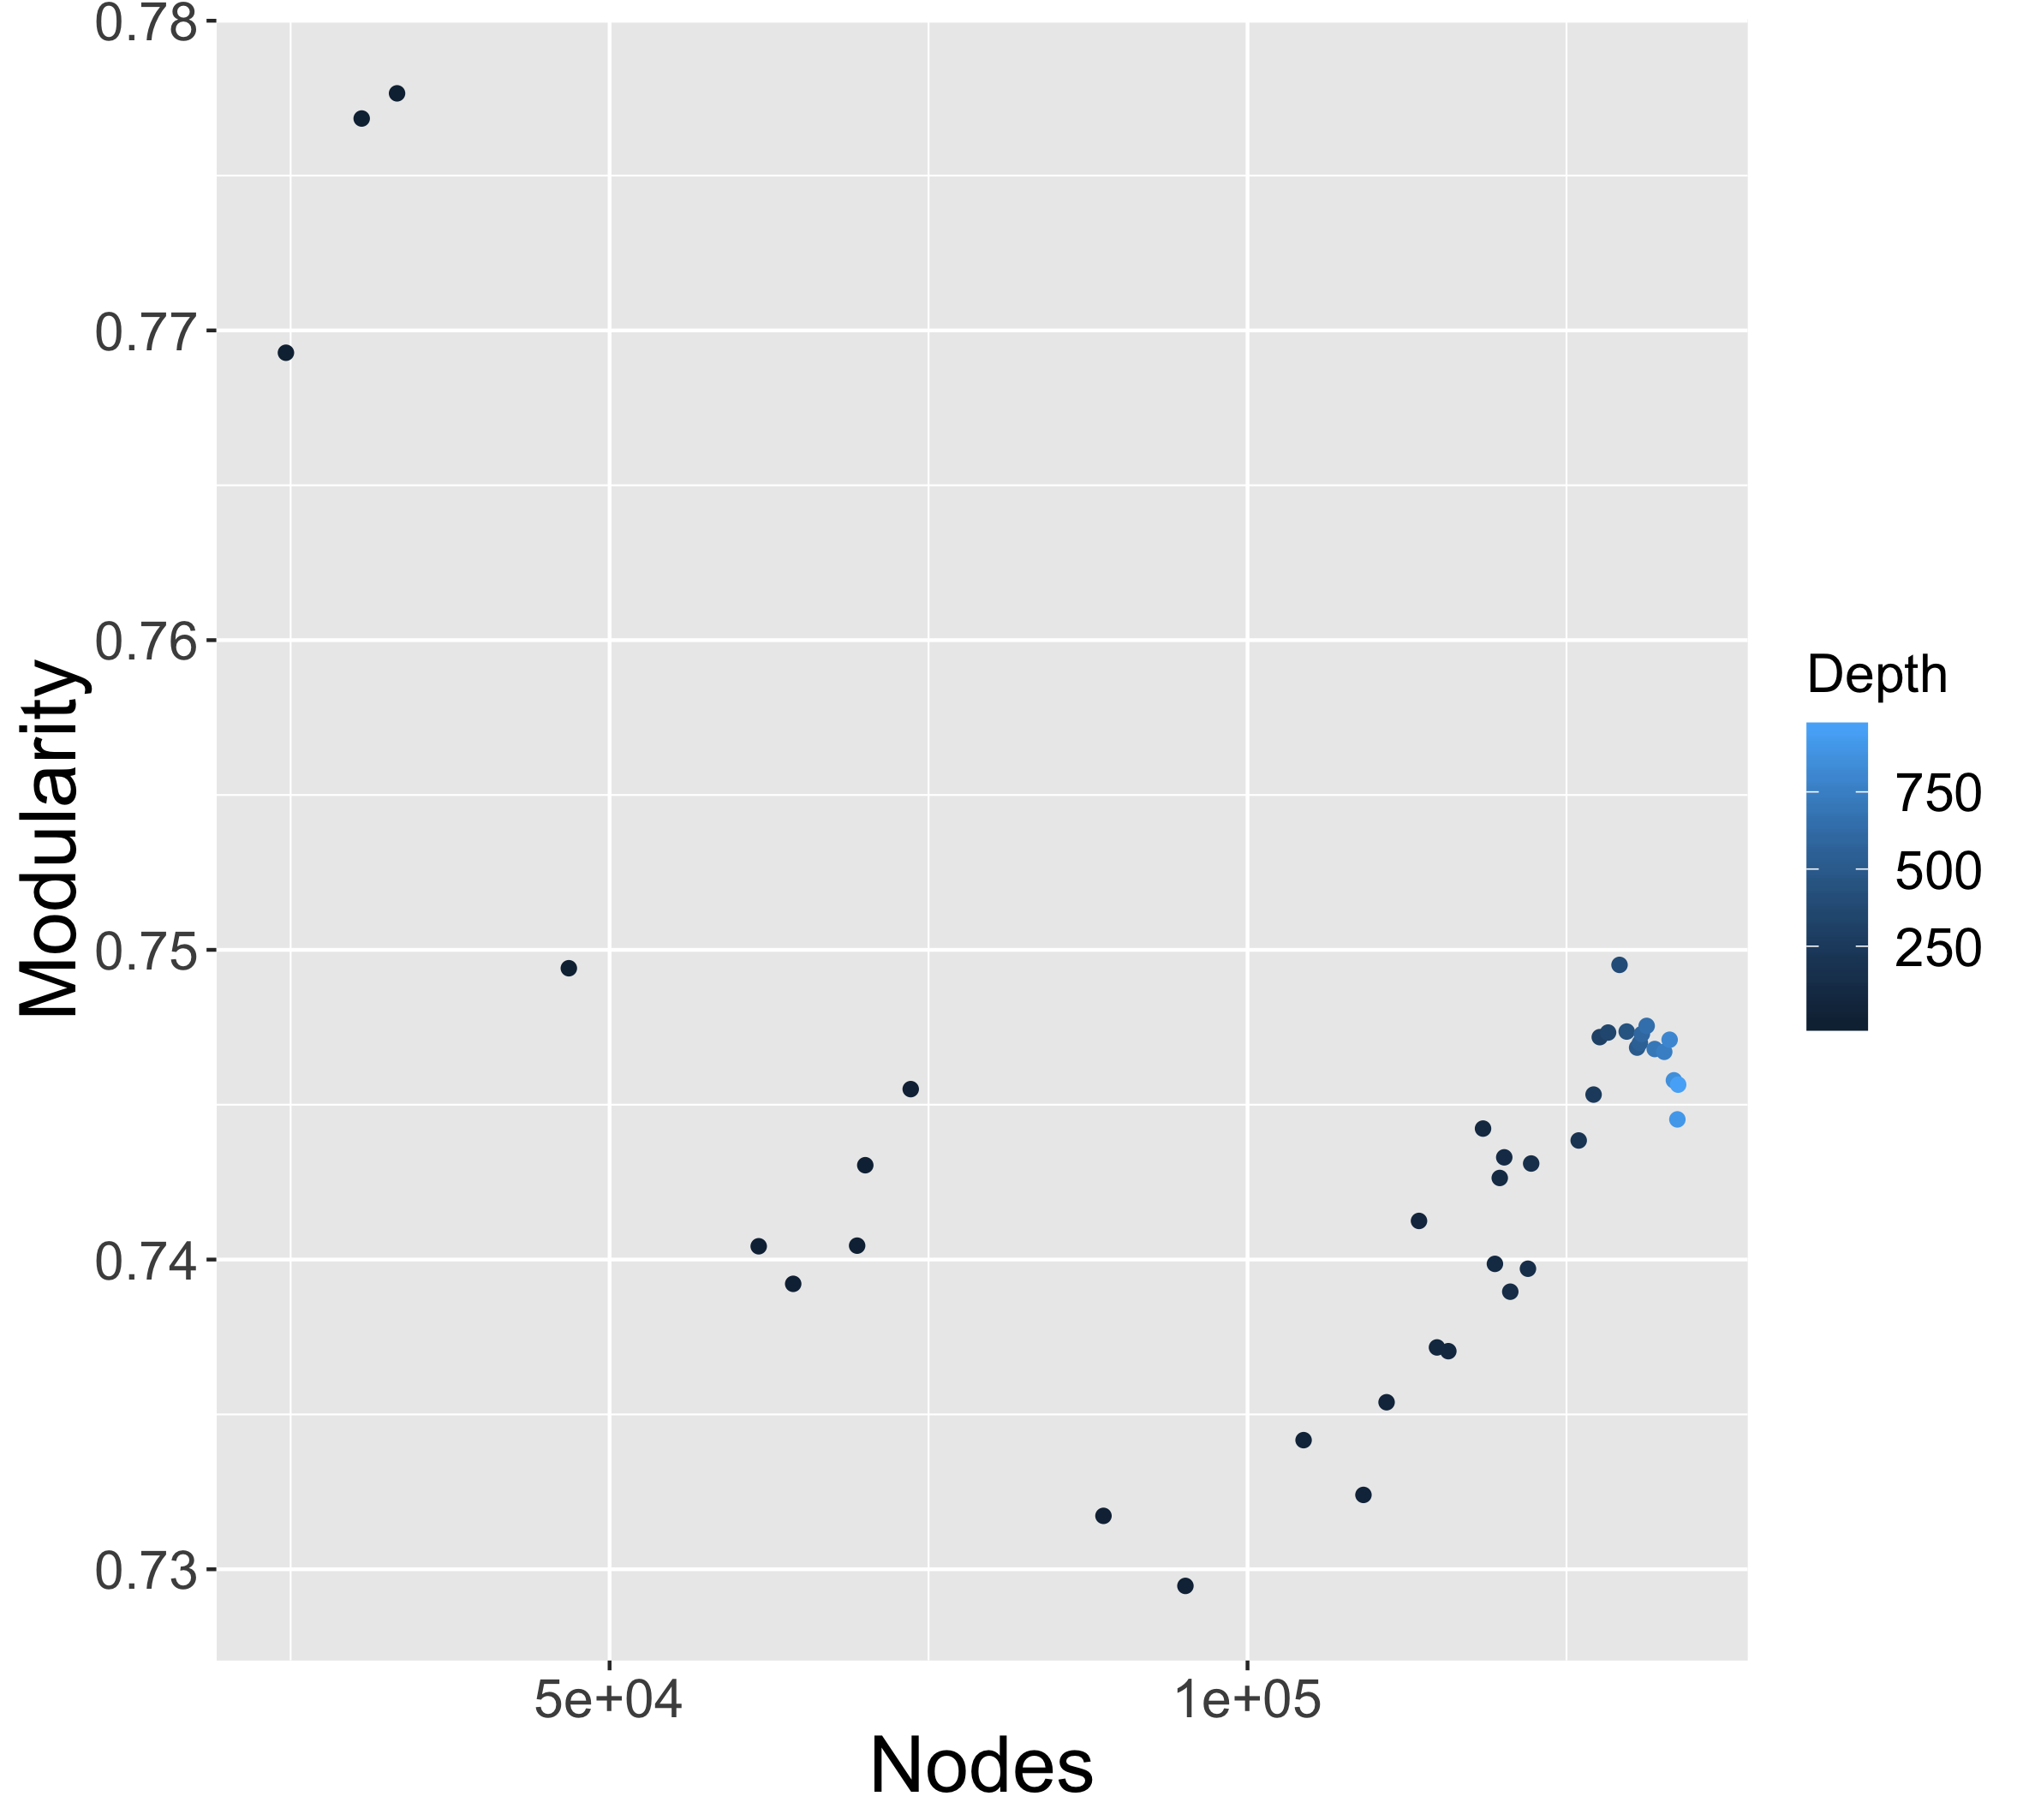
\includegraphics[height=0.8\textheight]{figures/pareto_vcount-modularity.png}

}



\sframe{Citation network}{

\centering
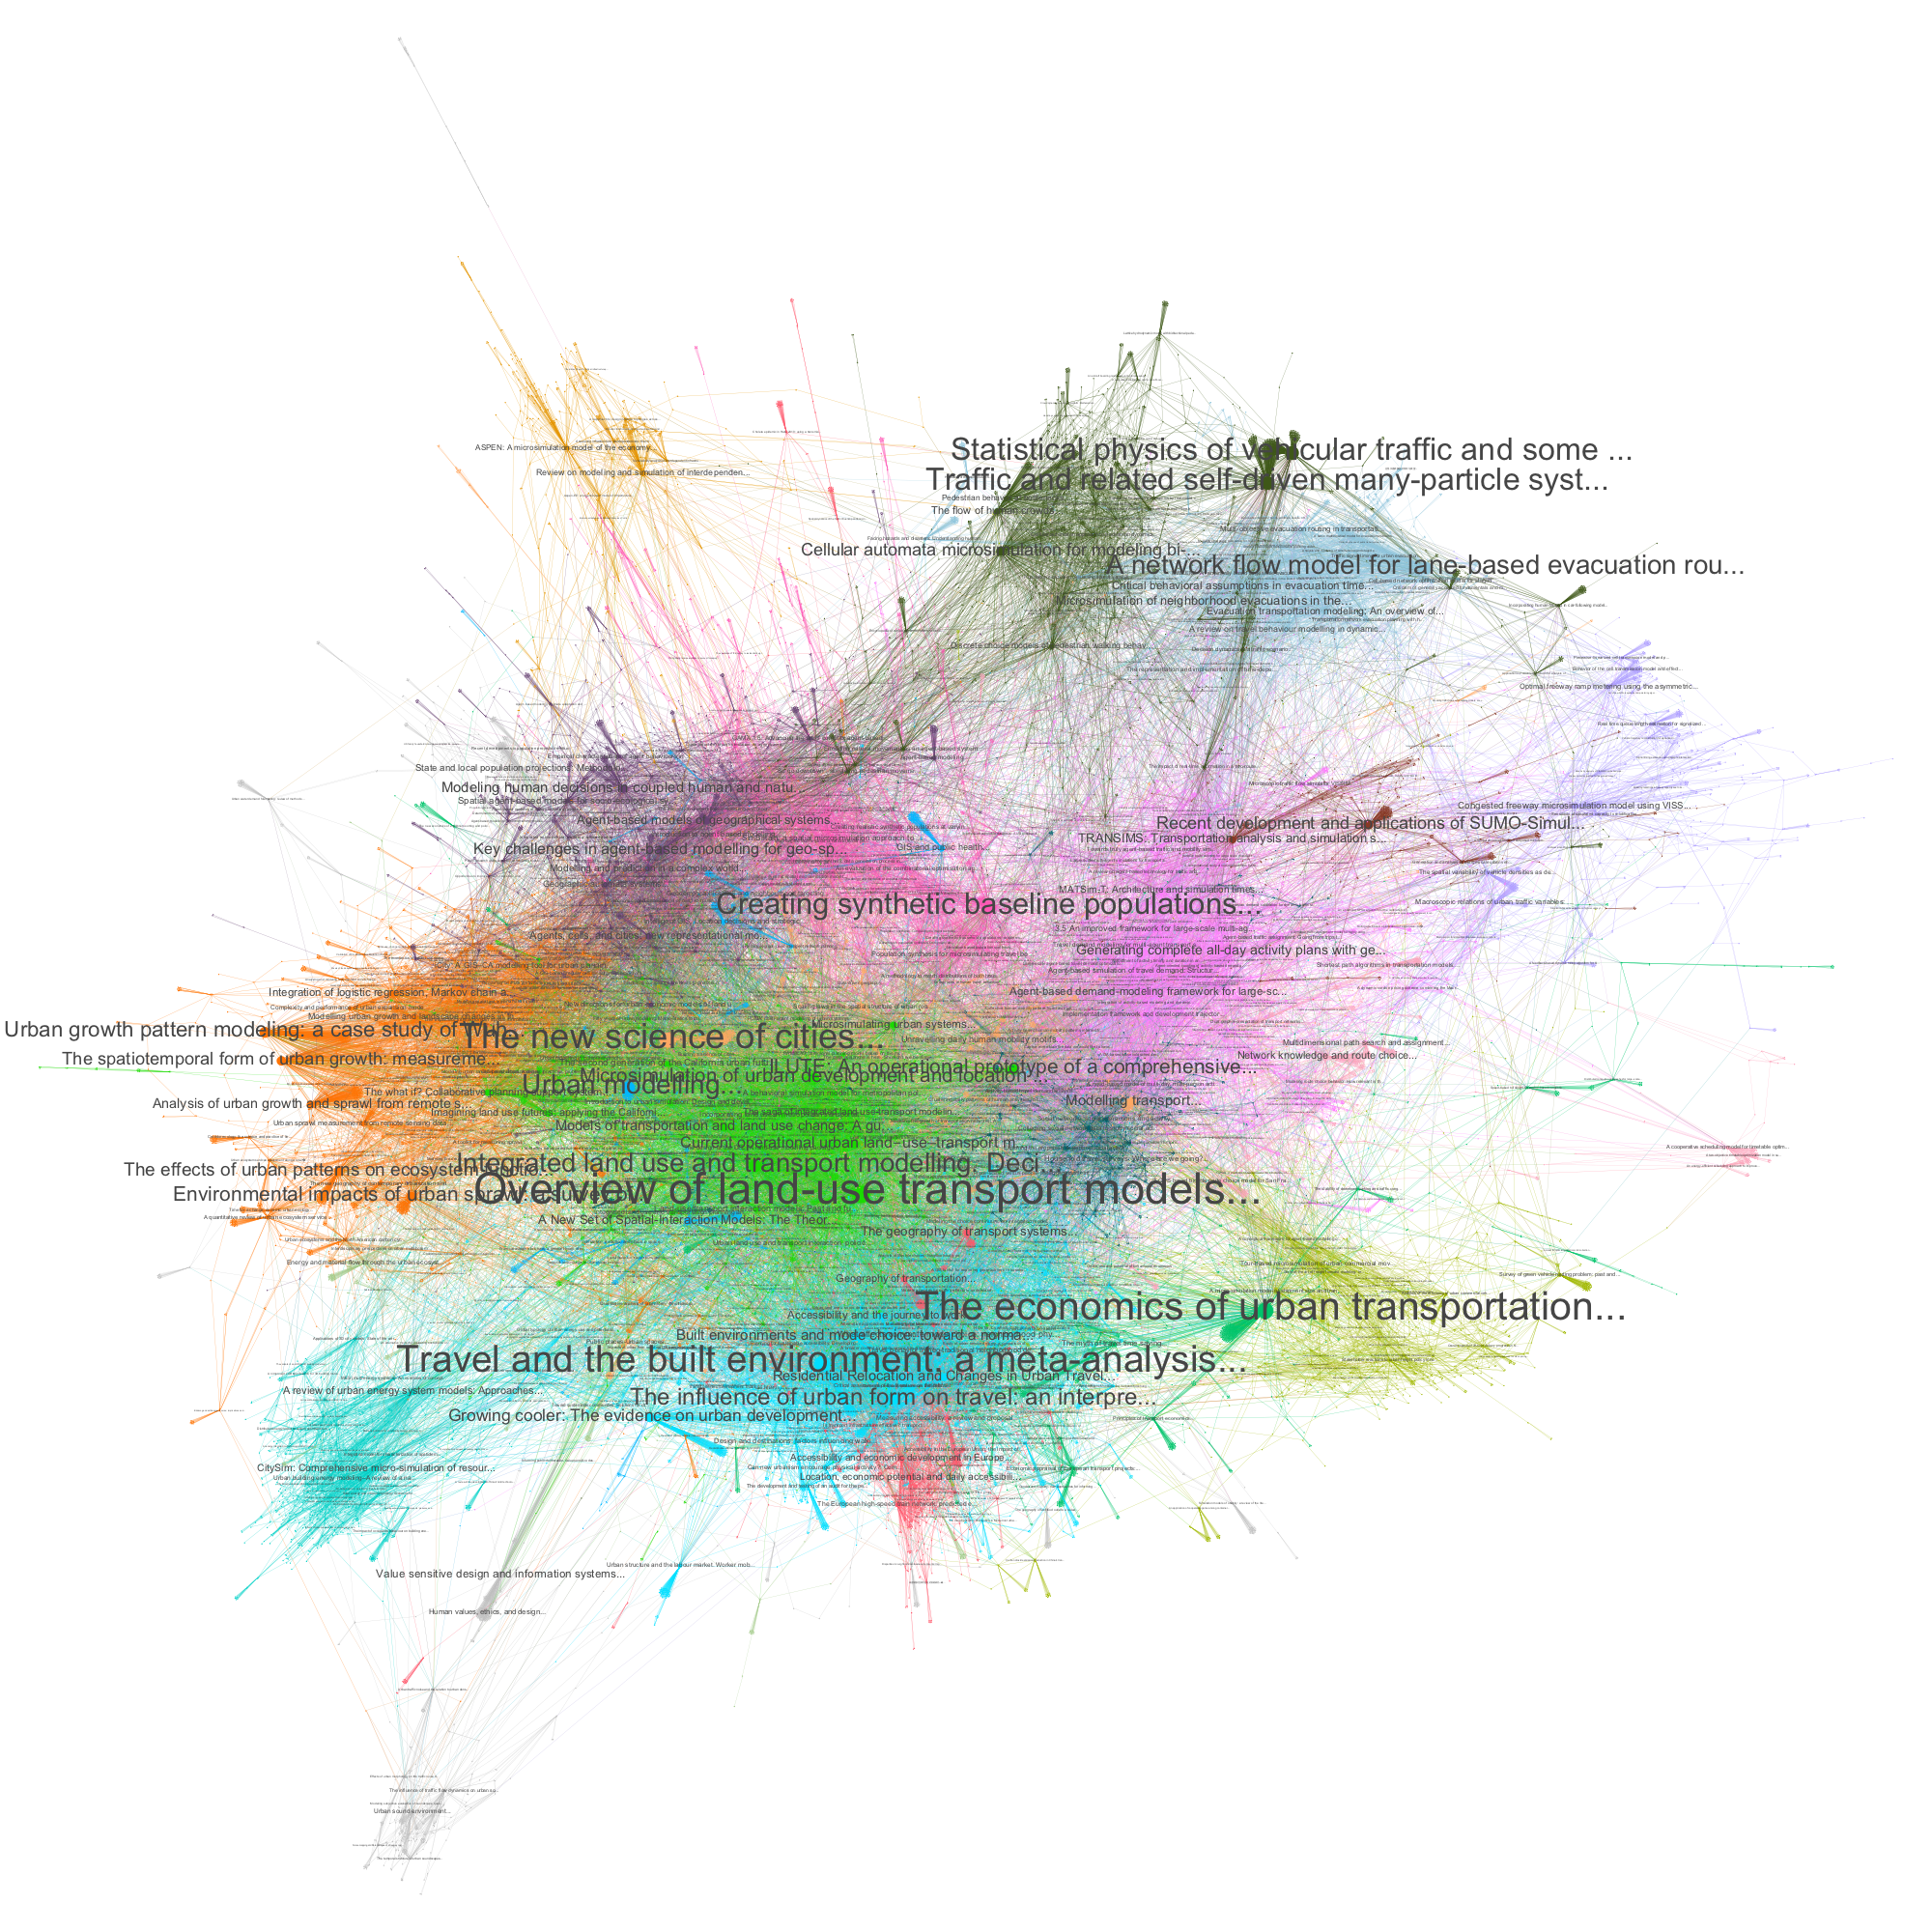
\includegraphics[width=1.05\textwidth,trim={0 0 0 8cm},clip]{figures/core_hdepth3_filtered_LOWRES.png}

}

\sframe{Core communities}{

\textit{Relative positioning of clusters of interest}

\centering

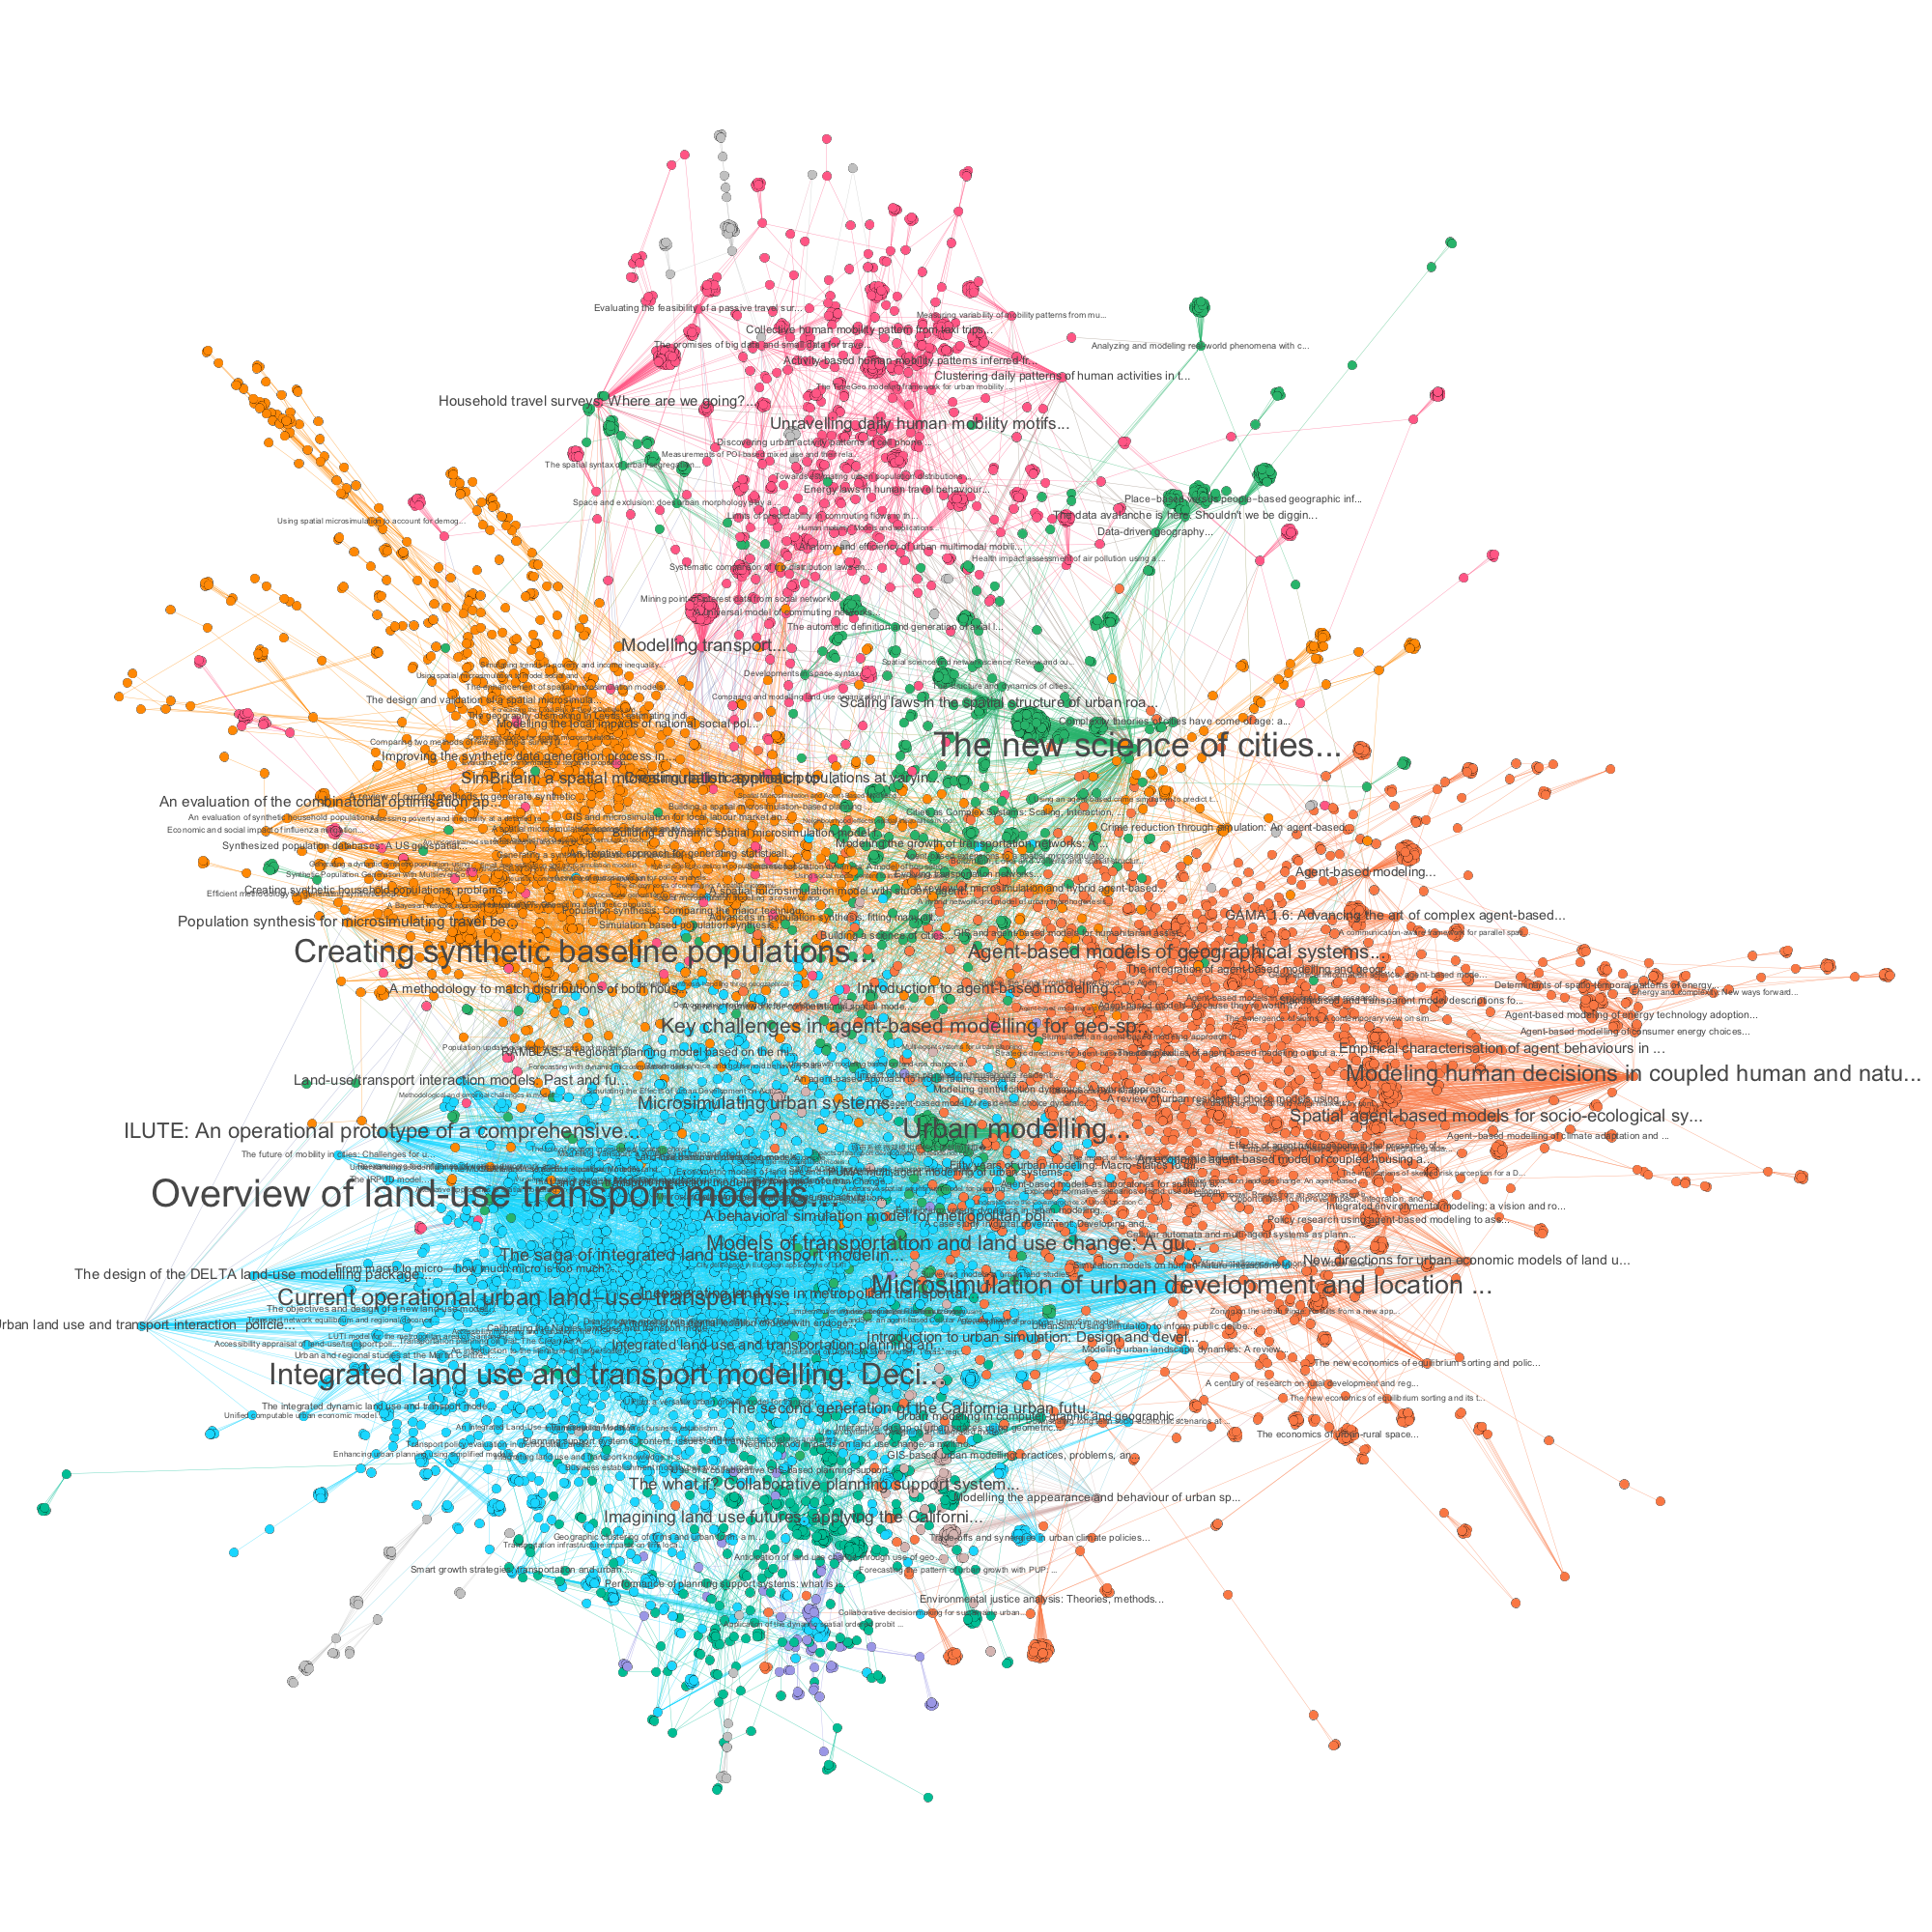
\includegraphics[height=0.9\textheight]{figures/core_hdepth3_filtered_targeted_LOWRES.png}

}


\sframe{Preliminary conclusions from literature mapping}{

\begin{enumerate}
	\item Robustness of collected citation network: relevance of keyword requests used
	\item Highly modular but connected networks: potential for more interdisciplinary bridges
	\item Complex systems (\cite{batty2013new}, scaling laws, network analysis) is a community and acts as a ``glue'' between different domains
	\item Work in progress: interdisciplinarity measures
	\item Work in progress by Maarten (confirms 3.): temporal evolution of network structure
\end{enumerate}

}



\section{Specific definitions of Microsimulation and ABM}

\sframe{Defining Microsimulation}{

\justify

\textit{In practice, microsimulation used very differently by different domains: transportation (e.g. VISSIM, or from TRANSSIMS to MATSIM), economics (taxes models), biological science, demographics, geography (ecology totally absent here, they use ``individual-based model'')}

\bigskip

Starting from our requests (mainly ``spatial microsimulation model''), we removed $\simeq 19\%$ (economics/finance and biological science) of nodes and get an ``urban modeling'' corpus covering a large span (including ABM and CA not present at the beginning)

\bigskip

$\rightarrow$ we can use the approach of demography/geography in a legitimate way when studying urban modeling   

}

\sframe{Microsimulation and agent-based modeling}{

% micro ontology ; linked to implementation choice ?
% discrete dynamical system for quant

We thus work in the context of the following features of agent-based modeling and microsimulation \cite{birkin2011spatial}:

\medskip

\begin{itemize}
	\item Same ontological level (individual agent, e.g. individual or household)
	\item Microsimulation generally uses population reconstruction (data-driven parametrization)
	\item Processes in microsimulation are generally based on \textit{transitions} (implemented as transition matrices/probabilities distribution) - while ABM simulate each agent
	\item ABM focus on stylized processes at the agent-level (heterogenous, autonomous, cognitive agents) and interactions between agents (nearly absent in Microsim)
	\item Validation methods are poorly developed for both
\end{itemize}

\medskip

\textit{QUANT is a LUTI, but what ``type'' ? discrete dynamical system ?}

\medskip

\footnotesize

[Remark: mixing function, thematics, methods in model description - impossibility of model typologies ? \cite{varenne2017theories} functional typologies is only partial]

}




\section{Description of SPENSER}

\sframe{General purpose of SPENSER}{

  Individual and household-level spatially explicit dynamic simulation of population (projective model)

  \medskip

  \textbf{Purpose: } test policies and scenarios at any level
  
  \medskip
  
  \textbf{Modules: }
  
  \begin{itemize}
    \item Data sources APIs (\textit{UKCensus}, \textit{UKSurvey}, \textit{UKPopulation}: uniformize population projections / test variants)
  	\item Synthetic population generator
  	\item Dynamic micro-simulation library
  	\item Simim, spatial interaction library
  \end{itemize}
  
  \medskip

  \textit{In practice, not yet integrated - libraries still being developed and do not seem to be all coupled. Typical use: use data sources to generate synthetic population, Simim to include the impact of a scenario, and simulate using the dynamic microsimulation.}
  
  % + use DAFNI for user interface / visualization / integration of HPC.
  
  \medskip
  
  \textit{DAFNI is used for (i) user-friendly scenario definition; (ii) distribution of simulations on high performance computing; (iii) visualization of simulation results. See example of Simim presented yesterday.}
  
}

\sframe{Flowchart of SPENSER}{

% can integrate ?

\Huge
\centering

\textit{SPENSER Flowchart}


}



\sframe{Synthetic population generation}{

%(Iterative Prop Fitting)

Library \textit{humanleague} generate synthetic population (population at the individual level from distribution of aggregated data) using:

\begin{itemize}
	\item Iterative Proportional Fitting (independent characteristic of individuals while respecting empirical marginals - issue of integerisation for individual populations)
	\item Quasi-random Integer Sampling (similar result but with a higher fidelity on generated population entropy, while IPF maximizes entropy)
	\item Combination of both (experimental ?)
\end{itemize}


}

\sframe{Iterative Proportional Fitting}{

\textit{Classical algorithm for IPF:}

\medskip

Let $x_{i_1 \ldots i_k}$ the multidimensional empirical table to fit, and $x_k = \sum_{\vec{i} = (i_{k'}), k'\neq k} x_{\vec{i}}$ the marginals to preserve.

Given initial values $y_{\vec{i}}^{(0)}$, then 

\[
y_{\vec{i}}^{(kt + k')} = \frac{y_{\vec{i}}^{(kt + k' - 1)}}{\sum y_{\vec{i}}^{(kt + k' - 1)}} \cdot x_{k'}
\]

converges to $y_{\vec{i}} = \prod_k \tilde{y}_k$ such that marginals are preserved and variables are independent.

}

\sframe{Quasi-random Integer Sampling}{

\textit{Issue with IPF: entropies of variables are maximized and integerization is needed (can introduce some bias)}

\bigskip

\cite{smith2017population} proposes to use data sampling without replacement and with quasi-random sequences (Sobol sequence - converge faster to estimate integrals) to tackle these issues:

\medskip

\begin{itemize}
	\item Take the marginals as empirical discrete multi-dimensional distribution
	\item Sample sequentially without-replacement and with a Sobol sequence from this distribution until the distribution is empty
\end{itemize}


}

\sframe{Dynamic microsimulation}{

Library \textit{neworder} is a generic cpp/python library for microsimulation.

\medskip

\begin{itemize}
	\item Framework to specify models in python: initialization, transitions (each having population as output)
	\item Statistical sampling methods included, as well as classical dataframe operations (e.g. randomly modify a column given a transition matrix), efficiently implemented in cpp
	\item Proof-of-concept for now (closest to SPENSER application): simulation of England and Wales population on 40 years with processes of birth, death and migration (internal and external)
\end{itemize}

}

\sframe{Spatial interactions}{

% concurrent of quant ? for pop only - migrations

Library \textit{simim} is a spatial interaction library for population migration

\medskip

\begin{itemize}
	\item Fit a spatial interaction model (globally constrained model) to migration data (also in time with population projections)
	\item Fitted model can be applied to study the impact of scenarios in infrastructure: housing project, employments, changes in attractiveness
	\item It is \textbf{not} a concurrent of QUANT (no transportation nor accessibility), rather a simpler alternative for scenario testing in QUANT $\rightarrow$ relevance of replacing it by QUANT
	\item Can be used for the desktop version of QUANT (Maarten currently testing ?)
\end{itemize}


}

\sframe{Technical aspects}{

	% python + cpp // quant developed by Maarten using simim library

	\begin{itemize}
		\item All the API are in python, so coupling will be easier with python models (similar to integration into DAFNI ?)
		\item cpp backend may make model embedding more difficult (need for containers)
		\item Regarding performance issues, blocking points are significantly different in QUANT (shortest paths and accessibility) and SPENSER (large populations synthesis and microsimulation)
	\end{itemize}
	

}



\section{Coupling QUANT and SPENSER: prospects}

% -> roadmap, incl sensitivity analysis

\sframe{Comparison of QUANT/SPENSER properties}{

%%%%%%%%%%%%
\begin{table}
\vspace{-0.5cm}
	\centering
	\begin{tabular}{|p{3.8cm}|p{3.5cm}|p{3.5cm}|}
	\hline
	\footnotesize
	& QUANT & SPENSER \\
	\hline
Time scale & 10 years & 40 years \\
Spatial scale & UK & UK \\
Spatial resolution & MSOA & MSOA \\
Agent granularity & Aggregated counts & individual level \\
Static/Dynamic & Equilibrium (static) & Dynamic \\
Randomness & Deterministic & Monte-Carlo \\\hline
Process: Transportation & 3 modes & NA \\
Process: Economic activities & Accessibility-based relocations & NA \\
Process: Demographics & NA & Data-driven \\
Process: Migration flows & Accessibility-based relocations & Data-driven \\
\hline
	\end{tabular}
\end{table}
%%%%%%%%%%%%

%\footnotesize

%\begin{itemize}
%\item $^{\ast 1}$ stylized time scale of metropolitan relocations \cite{wegener2004land}
%      \item $^{\ast 2}$ model structure is however stationary - this is an important issue for a possible application to 2070
%      \item $^{\ast 3}$ discrete choice for transportation mode is not implemented in QUANT 
%      \item $^{\ast 4}$ probabilities of basic demographic events (ageing, mortality, fertility, household formation, health, migration) are computed from data
%\end{itemize}


}

\sframe{Alternatives for coupling}{

% \item Weak coupling Luti $\rightarrow$ microsimulation: using sequentially outputs of Quant as inputs of Moses. For example, evaluating a new transportation scenario will provide predictions for new populations, employments and commuting flows. Distributing the synthetic population and its movements conditionally to this new distribution (respecting reasonably some statistical properties of the original data, what may pose difficult synthetic data generation problems), and running the microsimulation model with this new parametrization, could provide micro-based measures of the impact of the new transportation line (e.g. exposure to pollution, access to health facilities, segregation, etc.). In that case, it does not seem to make much sense to use the aggregated prediction of the microsimulation model, since the uncertainty on input data will be high as a output of the upstream model (``\textit{garbage in-garbage out}''), and the coupled model has a prospective and scenario-testing function.
%\item Weak coupling Microsimulation $\rightarrow$ Luti: the other way around, population projections obtained with microsimulation, which should be more precise than relocations by Quant (assuming that the system remains stationary and that exogenous effects are reasonably included), can be used as an input of the Quant model, in order to apply it in future times when for example planning long term infrastructure projects. More accurate future populations will provide more accurate generalized accessibility projections given or not some modification of the transportation network. The question answered and model function would also be territorial prospective. %(\textit{Open question : how do model functions in the sense of the typology of \cite{varenne2017theories} evolve during model coupling, do some typical patterns exist or is it case/scale specific ? Given a ``strength'' of models (a partial order on a subset of models given some objectives), are there patterns on the strength of the coupled model ?})
%\item Both previous proposition make sense assuming large approximations and assumptions. However, assuming in the first case that population statistical properties remain similar after urban changes is not accurate, as the composition of population or their behavior may drastically change. In the second case, assuming that population projections do not depend much on the changes in the accessibility landscape is also not accurate. A strong coupling Microsimulation $\rightarrow$ Luti, in a sense a co-evolutive model between  demographic dynamics and dynamics of accessibility in terms of transportation, population and jobs, would object to these two inaccuracies and in theory be more appropriate. It would provide both applications, i.e. population exposure impacts of transport and land-use scenarios, but also accurate projections and planning. This being said, this approach must be taken with caution. Very few co-evolution models of territorial systems (whatever the objects studied) do exist in the literature, and the problem remains relatively opened methodologically, theoretically and empirically (e.g. \cite{raimbault2018modeling} extended the city system model of \cite{raimbault2018indirect} to provide a co-evolution model between transportation networks and territories at the macro-scale, which although very novel as such kind of models remains very simple and highly limited). For example, one can use Quant population dynamics to constraint microsimulation probabilities at fixed time steps, or one can on the contrary use microsimulation outputs as additional exogenous constraints for Quant which will be useful to redistribute employments and a given transportation scenario on a long time period. Many different coupling choices must be more thoroughly listed, studied and possibly compared. In that sense, building a strongly coupled model is similar to constructing a new model.

Possible couplings:

\medskip

\begin{itemize}
	\item Weak coupling Luti $\rightarrow$ microsimulation: \textit{using demographic output of QUANT as the migration module of SPENSER - i.e. replacing the SIMIM module}
	\item Weak coupling Microsimulation $\rightarrow$ Luti: \textit{using demographic output of SPENSER as input of QUANT - useful to ``run QUANT in the future''}
	\item Strong coupling: as much choices as potential ``coupling processes'' (examples next slide)
	% iteration in time and/or during model iterations of interactions between inputs/outputs
\end{itemize}


\medskip

$\rightarrow$ technically achieve one weak coupling is a first requirement before attempting anything else; this imposes sensitivity analysis to be sure we get information from the coupling

$\rightarrow$ strong coupling can be seen as building a new model: specific ontologies and processes for how iterative inputs/outputs interact
% I have string doubts about the relevance of the latest as soon as we do not know very well the behavior of everything

}

\sframe{Strong coupling}{

Examples of ``coupling ontologies'':

\medskip

\begin{itemize} 
    \item run QUANT each $\tau$ years with SPENSER input to include infrastructure and employment changes given projected transportation scenarios, and thus modification in population initial state of next SPENCER
	\item similar coupling, but taking into account modification of jobs out of QUANT to impact SPENSER migration matrix (\textit{need an additional model})
	\item run QUANT each year with job/infrastructure modifications (with job projections or fixed) to ``recalibrate'' SPENSER
	\item \ldots
\end{itemize}

}


\sframe{Example of strong (multi-scale) model coupling}{
  
  % (i) population differences are computed by the interaction model; (ii) top-down feedback modifies parameters of mesoscopic models, given control parameters to capture typical scenarios (transit-oriented development or sprawl for diffusion, metropolization or uniformization for aggregation); (iii) local urban form are evolved with the reaction-diffusion models at a given speed conditionally to the population variations; (iv) changes in urban form influence macroscopic interaction ranges (capturing the impact of local activity on global insertion), by integrating gravity flows in the area with a squared cost function making a compromise between congestion and flows
  
  \justify
  
  Coupling a system of city model \cite{raimbault2018indirect} with a reaction-diffusion local morphogenesis model \cite{raimbault2018calibration} involves supplementary ontologies: how does the macroscopic trajectory of a city influences its urban form parameters (here: stylized policies TOD/sprawl, clusters/uniformization) ? how does the changes in urban form modify macroscopic parameters (here: compromise between congestion and efficiency) ?
  
  \bigskip
  
  \centering
  
  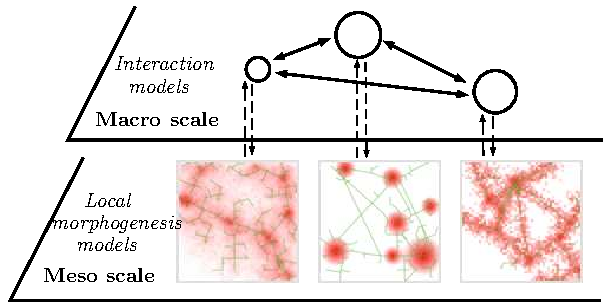
\includegraphics[height=0.5\textheight]{figures/multiscale_morph}
  
  
}



\section{Sensitivity analysis and OpenMOLE}

% incl description of OpenMOLE


\sframe{Sensitivity analysis of SPENSER}{
 
  % validation of spatial interaction module -> currently done by Maarten
  
  % done eitherway by the spenser team through dafni ?
 
 \textit{How robust are SPENSER outputs to noise ? Does SPENSER actually does something ? [already had the case of a model so data-driven it did nothing !]}
 
 \bigskip
 
 $\rightarrow$ Currently done by Nik and Andrew: stochastic sensitivity, sensitivity to input data (noise ?)
 
 \medskip
 
 $\rightarrow$ Currently done by Maarten: testing simim
 
}

\sframe{Sensitivity analysis of QUANT}{
  
  % ideas to go with : missing data / data perturbations
  %. => descruption of spatialdata / forcity / spatial projects generator
  
  \textit{How are QUANT output influenced by data / urban structure / accessibility patterns ?}
  
  \bigskip
  
  $\rightarrow$ synthetic perturbation of initial pop/job distributions
  
  \medskip
  
  $\rightarrow$ synthetic perturbation of transportation network
  
  \medskip
  
  $\rightarrow$ run QUANT on synthetic city systems
  
  \medskip
  
  \textit{All implemented into the scala library } \texttt{spatialdata} \textit{and included as sensitivity analysis methods into OpenMOLE}
  
}


\sframe{Computational experiments using OpenMOLE}{

 % what is openmole
 % what does it do
 % demo ?
 
 OpenMOLE is an open-source and free software developed at the Complex Systems Institute in Paris to
 
 \medskip
 
 \begin{itemize}
 	\item Embed any model in numerical experiments
 	\item Provide transparent to state-of-art model validation methods
 	\item Provide transparent access to high performance computing environments
 \end{itemize}

\medskip

With an easy to access DSL built on scala, available even to modelers with less strong computer science skills

\medskip

\textit{demo}

}


\sframe{Model exploration methods}{

% list of methods
  
  \textit{Currently available in OpenMOLE:}
  
  \medskip
  
  \begin{itemize}
  	\item Design of Experiments (explicit sampling, one factor at a time, grid sampling, Latin Hypercube sampling, Sobol sequences)
  	\item Spatial synthetic data sampling
  	\item Global sensitivity analysis (Morris and Saltelli methods)
  	\item Model calibration (NSGA2)
  	\item Diversity search, parameter profile
  	\item Bayesian calibration (Approximate Bayesian Calibration)
  	\item Inverse problem
  \end{itemize}
  
  
  
  \bigskip
  
  \textit{Currently being developed:}
  
  \begin{itemize}
  	\item Monte Carlo Markov Chain methods, Simulated Method of Moments, Simulated Annealing-RJMCMC
  	\item Hybrid Kalman NSGA2 for calibration of noisy models
  	\item Many-objectives optimization: NSGA3
  \end{itemize}
  
}


\sframe{Possible difficulties with DAFNI}{
  
  % disclaimer : kind of a priori judgement from what we only saw yesterday
  
  % - no work on model epistemology (worse : constraining format on models and data)
  % - no theoretical / empirical work on model coupling (definition of a coupling ?)
  % - no work on model validation / calibration
  % - how much HPC ? coupling with EGI ?
  
  \textit{Questions I could not ask yesterday / a priori judgement from what we saw:}
  
  \begin{itemize}
  	\item No work on modeling epistemology / model diversity - on the contrary seems constraining on model and data format
  	\item No theoretical nor empirical research (yet, but research program either ?) on model coupling (definition of coupling, relevance, etc.) [not sure on the heterogenous model embedding part also - the \texttt{smif} library only includes python models]
  	\item No specific work on model validation and calibration, integration of methods
  	\item How much HPC is actually provided ? (could a local slurm be better ?) Resource sharing with other initiatives such as EGI ?
  \end{itemize}
  
}

\sframe{Running OpenMOLE on DAFNI}{

 % possibility to run as a service ? (kubernetes cluster - currently also being intergaetd
 % 

 DAFNI allows the creation and management of kubernetes clusters
 
 $\rightarrow$ possible use of OpenMOLE multi-user deployment currently being finalized
 
 \bigskip
 
 DAFNI provides services such as Jupyter
 
 $\rightarrow$ possibility to include OpenMOLE as a service (complementarity of exploration methods and easier embedding, rudimentary workflow language and model embedding already in DAFNI)

}


\sframe{Conclusion: roadmap}{

 In conclusion: coupling LUTI and microsimulation is relevant but must be done step by step and carefully.
 
 \bigskip
 
 Proposed roadmap:
 
 \begin{itemize}
 	\item Fall: sensitivity analysis on both sides
 	\item January: Weak couplings
 	\item Later: experiments with strong couplings
 \end{itemize}



}




%%%%%%%%%%%%%%%%%%%%%
\begin{frame}[allowframebreaks]
\frametitle{References}
\bibliographystyle{apalike}
\bibliography{biblio}
\end{frame}
%%%%%%%%%%%%%%%%%%%%%%%%%%%%










\end{document}







